\chapter{Fundamentação Teórica}
\label{cap:fund_teorica}

\section{Métodos de Análise de Séries Temporais}
\label{sec:dmc}

O coeficiente \pdcca~\cite{Zebende2011} foi formulado tendo como bases o \emph{Detrended Fluctuation Analysis} (DFA)~\cite{Peng_1994} e o \emph{Detrended Cross-Correlation Analysis} (DCCA)~\cite{Podobnik2008}. O DFA é um método de análise de uma série temporal que fornece um parâmetro de auto-afinidade. O termo \emph{Detrended} refere-se a eliminação de uma tendência. O processo é executado em 6 passos:

\begin{enumerate}
    \label{dfa}
    \item Pegando a série temporal \(\{x_{i}\}\) com  \(i\) variando de  \(1\) à \(N\), a série integrada \(X_{k}\) é calculada por \(X_{k} = \sum_{i=1}^{k}\left[x_{i} - \langle x \rangle \right] \) com \(k\) também variando entre \(1\) e \(N\);
    \item A série  \(X_{k}\) e dividida em \(N - n\) caixas de tamanha\(n\) (escala temporal), cada caixa contendo \(n + 1\) observações, iniciando em \(i\) até \(i + n\);
    \item Para cada caixa um polinômio (geralmente de grau 1) é ajustado, gerando \(\widetilde{X}_{k, i}\) with \( i \le k \le (i + n) \) eliminando assim a tendência (detrended values);
    \item  para cada caixa é calculado: \(f_{DFA}^{2}(n, i) = \frac{1}{1+n} \sum_{k=i}^{i + n}(X_{k}-\widetilde{X}_{k, i})^{2}\)
    \item Para todas as caixas de umaescala temporal o DFA é calculado como: \(F_{DFA}(n) = \sqrt{\frac{1}{N - n} \sum_{i=1}^{N-n} f_{DFA}^{2}(n, i)}\);
    \item Para um número de diferentes escalas temorais (n), com valores possíveis entre \( 4 \le n \le \frac{N}{4}\), a função \(F_{DFA}\) é calculada para encontrar a relação entre \(F_{DFA} \times n\)
  \end{enumerate}

DFA também  representa as propriedades de auto-correlação de longo alcance de uma lei de potência~\cite{Zebende2013}. Se a correlação não existe, ou é uma correlação de curto alcance o valor do parâmetro \(\alpha = 0.5\), \(\alpha < 0.5\) indica antipersistência e \(\alpha > 0.5\) persistência.

O \(DCCA\) generaliza o DFA para estabelecer a correlação entre duas séries temporais \cite{Podobnik2008}. O valor deste coeficiente tende a ser a média dos valores do DFA das duas séries. 

Este coeficiente \(\lambda\) indica a existência de uma correlação entre duas séries regidas por leis de potência, mas não quantifica o nível desta correlação. O \emph{Detrended cross-correlation coefficient} ou \pdcca (equação \ref{eq_pdcca}) é um coeficiente que, variando entre -1 e 1, aponta ausência de correlação cruzada para valores próximos de zero, sendo maior a correlação quanto mais o valor se aproximar de 1 e maior a antecorrelação quanto mais o valor se aproximar de -1~\cite{Zebende2011}. 

\begin{equation}
\label{eq_pdcca}
\rho DCCA(n) = \frac{F_{DCCA}^2 (n)}{ F_{DFA1} (n) F_{DFA2} (n)}
\end{equation}

O método foi estatisticamente validado~\cite{PhysRevE.84.066118}, testado~\cite{vassolerZebende2012, Guedes2017, Ferreira2018},
e critérios para avaliação de relevância estatísticas do resultados foram desenvolvidos~\cite{Guedes2018,Guedes2018a}.

O \pdcca~foi estendido para calcular a correlação cruzada de múltiplas series temporais. Denominado \emph{Detrended Multiple Cross-Correlation Coefficient}~(\dmc), representa a generalização do \pdcca para múltiplas variáveis~\cite{Zebende2018}. Implementado com abordagem de janelas móveis~\cite{Guedes2021} e foi desenvolvido um teste estatístico para o coeficiente múltiplo~\cite{DaSilvaFilho2021}

Já que muitos dos problemas que envolvem sistemas complexos lidam com mais de uma variável independente. E os sistemas e AM costumam abordar múltiplas variáveis independentes em suas buscas por padrões, dentre os métodos correlatos ao \pdcca, o \dmc apresenta as qualidades mais promissoras para embasar um algoritmo de AM.

\section{Aprendizado de Máquina e Redes Neurais Artificiais}
\label{sec:ml}

O aprendizado de máquina consiste na aplicação de algoritmos capazes de, através do processamento de um grande conjunto de dados, encontrar padrões, generalizar os critérios de encontrar padrões e prever eventos futuros\cite{bendavid2014}.

\begin{figure}[!htb]
	\centering
	\caption{Aprendizado de Máquina- diagrama conceitual}
	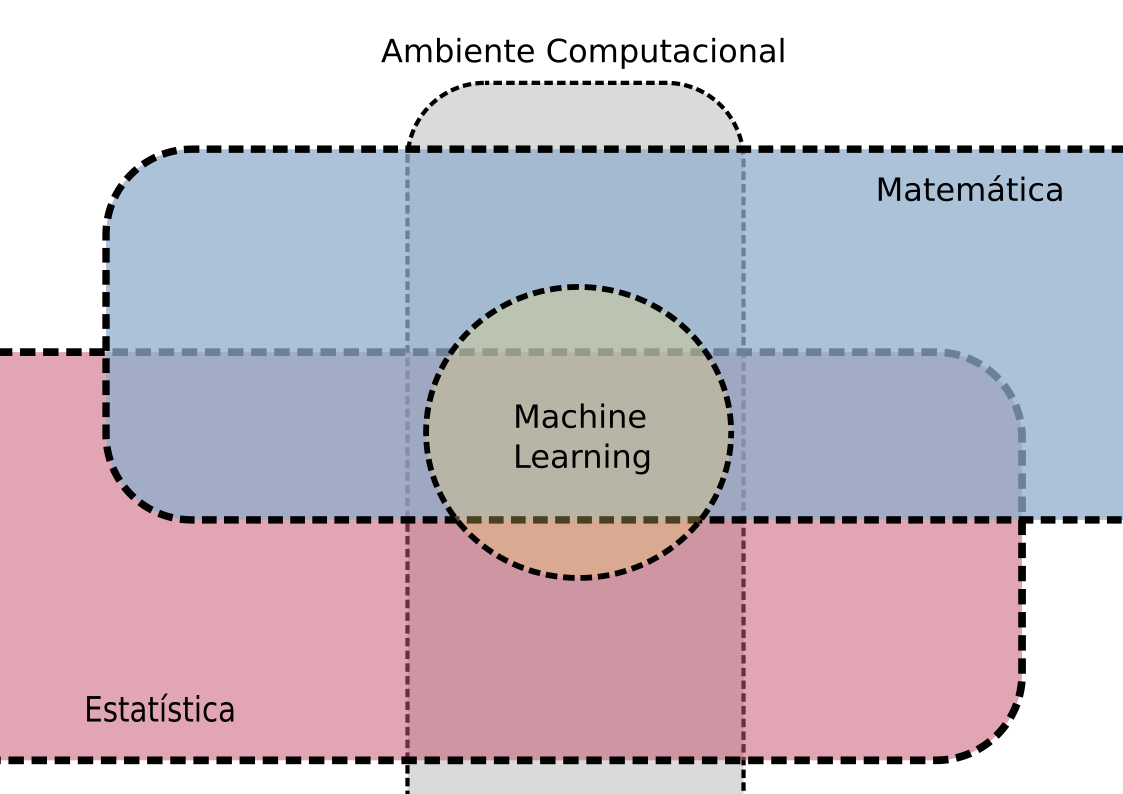
\includegraphics[width=.7\textwidth]{../Figures/ML/mat_est_ML.png}
	\\{\footnotesize Fonte: Elaborada Pelos Autores}
	\label{fig:MLdiag}
\end{figure}

Um campo guiado pela experimentação prática \cite{bishop2006}, pode ser definido pela busca em melhorar o desempenho computacional na realização de uma tarefa, através da experiência \cite{mitchell1997}. O desempenho nesta definição refere-se principalmente a quantificação dos acertos de acordo com uma métrica adequada à resolução do problema em questão e a experiência refere-se a um conjunto de dados coletados.

As tarefas em que os métodos de ML costumam superar os outros algoritmos também apresentam características peculiares: tratam de problemas fracamente definidos do ponto de vista matemático e/ou cujos métodos de resolução matemática são muito custosos do ponto de vista computacional em relação à velocidade necessária para a solução do problema na prática.

Reconhecimento facial e outras formas de interpretação de imagens, máquinas que andam, nadam e dirigem veículos, processamento de linguagem natural (falada e escrita) são exemplos de problemas fracamente definidos. Como definir com instruções de programação convencionais a sequência de instruções necessárias para ensinar um computador a resolver um dos destes problemas? Os algoritmos de ML tem apresentado boas respostas para este tipo de problema.

